

\bta{2006}

\section{Use of English}

\noindent
\textbf{Directions:}\\
Read the following text. Choose the best word (s) for each
	numbered blank and mark A, B, C or D on ANSWER
	SHEET. (10 points)


\TiGanSpace


The homeless make up a growing percentage of America's
population. \cloze , homelessness has reached such proportions
that local governments can't possibly \cloze. To help homeless
people \cloze independence, the federal government must support
job training programs, \cloze the minimum wage, and fund more
low-cost housing.

\cloze everyone agrees on the number of Americans who are
homeless. Estimates \cloze anywhere from 600,000 to 3
million. \cloze the figure may vary, analysts do agree on another
matter: that the number of the homeless is \cloze. One of the
federal government's studies \cloze that the number of the
homeless will reach nearly 19 million by the end of this decade.

Finding ways to \cloze this growing homeless population has
become increasingly difficult. \cloze when homeless individuals
manage to find a \cloze that will give them three meals a day
and a place to sleep at night, a good number still spend the bulk of
each day \cloze the street. Part of the problem is that many
homeless adults are addicted to alcohol or drugs. And a significant
number of the homeless have serious mental disorders. Many
others, \cloze not addicted or mentally ill, simply lack the
everyday \cloze skills needed to turn their
lives \cloze. \emph{Boston Globe} reporter Chris Reidy notes
that the situation will improve only when there
are \cloze programs that address the many needs of the
homeless. \cloze Edward Zlotkowski, director of community
service at Bentley College in Massachusetts, \cloze it, ``There
has to be \cloze of programs. What's needed is a package deal.''


\newpage
\begin{enumerate}
	%\renewcommand{\labelenumi}{\arabic{enumi}.}
	% A(\Alph) a(\alph) I(\Roman) i(\roman) 1(\arabic)
	%设定全局标号series=example	%引用全局变量resume=example
	%[topsep=-0.3em,parsep=-0.3em,itemsep=-0.3em,partopsep=-0.3em]
	%可使用leftmargin调整列表环境左边的空白长度 [leftmargin=0em]
	\item
\fourchoices
{Indeed}
{Likewise}
{Therefore}
{Furthermore}




\item
\fourchoices
{stand}
{cope}
{approve}
{retain}




\item
\fourchoices
{in}
{for}
{with}
{toward}




\item
\fourchoices
{raise}
{add}
{take}
{keep}




\item

\fourchoices
{Generally}
{Almost}
{Hardly}
{Not}




\item

\fourchoices
{cover}
{change}
{range}
{differ}




\item

\fourchoices
{Now that}
{Although}
{Provided}
{Except that}




\item
\fourchoices
{inflating}
{expanding}
{increasing}
{extending}




\item
\fourchoices
{predicts}
{displays}
{proves}
{discovers}




\item
\fourchoices
{assist}
{track}
{sustain}
{dismiss}




\item

\fourchoices
{Hence}
{But}
{Even}
{Only}




\item

\fourchoices
{lodging}
{shelter}
{dwelling}
{house}




\item
\fourchoices
{searching}
{strolling}
{crowding}
{wandering}



\item

\fourchoices
{when}
{once}
{while}
{whereas}




\item

\fourchoices
{life}
{existence}
{survival}
{maintenance}




\item

\fourchoices
{around}
{over}
{on}
{up}




\item
\fourchoices
{complex}
{comprehensive}
{complementary}
{compensating}



\item

\fourchoices
{So}
{Since}
{As}
{Thus}




\item

\fourchoices
{puts}
{interprets}
{assumes}
{makes}




\item
\fourchoices
{supervision}
{manipulation}
{regulation}
{coordination}

\end{enumerate}

\vfil

\section{Reading Comprehension}



\noindent
\textbf{Part A}\\
\textbf{Directions:}\\
Read the following four texts. Answer the questions below each
text by choosing A, B, C, or D  Mark your
answers on ANSWER SHEET. (40 points)



\newpage
\subsection{Text 1}


In spite of  ``endless talk of difference,'' American society is an
amazing machine for homogenizing people. There is ``the democratizing
uniformity of dress and discourse, and the casualness and absence of
deference'' characteristic of popular culture. People are absorbed into
``a culture of consumption'' launched by the 19 th-century department
stores that offered ``vast arrays of goods in an elegant atmosphere.
Instead of intimate shops catering to a knowledgeable elite'' these were
stores ``anyone could enter, regardless of class or background. This
turned shopping into a public and democratic act.'' The mass media,
advertising and sports are other forces for homogenization.

Immigrants are quickly fitting into this common culture, which may not
be altogether elevating but is hardly poisonous. Writing for the
National Immigration Forum, Gregory Rodriguez reports that today's
immigration is neither at unprecedented levels nor resistant to
assimilation. In 1998 immigrants were 9.8 percent of the population; in
1900, 13.6 percent. In the 10 years prior to 1990, 3.1 immigrants
arrived for every 1, 000 residents; in the 10 years prior to 1890, 9.2
for every 1, 000. Now, consider three indices of assimilation---language,
home ownership and intermarriage.

The 1990 Census revealed that ``a majority of immigrants from each of
the fifteen most common countries of origin spoke English `well' or
`very well' after ten years of residence.'' The children of immigrants
tend to be bilingual and proficient in English. ``By the third
generation, the original language is lost in the majority of immigrant
families.'' Hence the description of America as a ``graveyard'' for
languages. By 1996 foreign-born immigrants who had arrived before 1970
had a home ownership rate of 75.6 percent, higher than the 69.8 percent
rate among native-born Americans.

Foreign-born Asians and Hispanics ``have higher rates of intermarriage
than do U.S.-born whites and blacks.'' By the third generation, one
third of Hispanic women are married to non-Hispanics, and 41 percent of
Asian-American women are married to non-Asians.

Rodriguez notes that children in remote villages around the world are
fans of superstars like Arnold Schwarzenegger and Garth Brooks, yet
``some Americans fear that immigrants living within the United States
remain somehow immune to the nation's assimilative power.''

Are there divisive issues and pockets of seething anger in America?
Indeed. It is big enough to have a bit of everything. But particularly
when viewed against America's turbulent past, today's social indices
hardly suggest a dark and deteriorating social environment.



\begin{enumerate}[resume]
	%\renewcommand{\labelenumi}{\arabic{enumi}.}
	% A(\Alph) a(\alph) I(\Roman) i(\roman) 1(\arabic)
	%设定全局标号series=example	%引用全局变量resume=example
	%[topsep=-0.3em,parsep=-0.3em,itemsep=-0.3em,partopsep=-0.3em]
	%可使用leftmargin调整列表环境左边的空白长度 [leftmargin=0em]
	\item
The word ``homogenizing'' (Line 2, Paragraph 1) most
probably means \lineread.

\fourchoices
{identifying}
{associating}
{assimilating}
{monopolizing}



\item
According to the author, the department stores of the 19th
century \lineread.

\fourchoices
{played a role in the spread of popular culture}
{became intimate shops for common consumers}
{satisfied the needs of a knowledgeable elite}
{owed its emergence to the culture of consumption}


\item
The text suggests that immigrants now in the U.S.
\lineread .

\fourchoices
{are resistant to homogenization}
{exert a great influence on American culture}
{are hardly a threat to the common culture}
{constitute the majority of the population}



\item
Why are Arnold Schwarzenegger and Garth Brooks mentioned in
Paragraph 5?

\fourchoices
{To prove their popularity around the world.}
{To reveal the public's fear of immigrants.}
{To give examples of successful immigrants.}
{To show the powerful influence of American culture.}



\item
 In the author's opinion, the absorption of immigrants into
American society is \lineread.

\fourchoices
{rewarding}
{successful}
{fruitless}
{harmful}


\end{enumerate}

\newpage
\subsection{Text 2}


Stratford-on-Avon, as we all know, has only one industry---William
Shakespeare---but there are two distinctly separate and increasingly
hostile branches. There is the Royal Shakespeare Company (RSC), which
presents superb productions of the plays at the Shakespeare Memorial
Theatre on the Avon. And there are the townsfolk who largely live off
the tourists who come, not to see the plays, but to look at Anne
Hathaway's Cottage, Shakespeare's birthplace and the other sights.

The worthy residents of Stratford doubt that the theatre adds a penny
to their revenue. They frankly dislike the RSC's actors, them with their
long hair and beards and sandals and noisiness. It's all deliciously
ironic when you consider that Shakespeare, who earns their living, was
himself an actor (with a beard) and did his share of noise-making.

The tourist streams are not entirely separate. The sightseers who come
by bus---and often take in Warwick Castle and Blenheim Palace on the
side---don't usually see the plays, and some of them are even surprised
to find a theatre in Stratford. However, the playgoers do manage a
little sight-seeing along with their playgoing. It is the playgoers, the
RSC contends, who bring in much of the town's revenue because they spend
the night (some of them four or five nights) pouring cash into the
hotels and restaurants. The sightseers can take in everything and get
out of town by nightfall.

The townsfolk don't see it this way and the local council does not
contribute directly to the subsidy of the Royal Shakespeare Company.
Stratford cries poor traditionally. Nevertheless every hotel in town
seems to be adding a new wing or cocktail lounge. Hilton is building its
own hotel there, which you may be sure will be decorated with Hamlet
Hamburger Bars, the Lear Lounge, the Banquo Banqueting Room, and so
forth, and will be very expensive.

Anyway, the townsfolk can't understand why the Royal Shakespeare Company
needs a subsidy. (The theatre has broken attendance records for three
years in a row. Last year its 1, 431 seats were 94 per cent occupied all
year long and this year they'll do better.) The reason, of course, is
that costs have rocketed and ticket prices have stayed low.

It would be a shame to raise prices too much because it would drive away
the young people who are Stratford's most attractive clientele. They
come entirely for the plays, not the sights. They all seem to look alike
(though they come from all over)---lean, pointed, dedicated faces,
wearing jeans and sandals, eating their buns and bedding down for the
night on the flagstones outside the theatre to buy the 20 seats and 80
standing-room tickets held for the sleepers and sold to them when the
box office opens at 10:30 a.m.


\begin{enumerate}[resume]
	%\renewcommand{\labelenumi}{\arabic{enumi}.}
	% A(\Alph) a(\alph) I(\Roman) i(\roman) 1(\arabic)
	%设定全局标号series=example	%引用全局变量resume=example
	%[topsep=-0.3em,parsep=-0.3em,itemsep=-0.3em,partopsep=-0.3em]
	%可使用leftmargin调整列表环境左边的空白长度 [leftmargin=0em]
	\item
From the first two paragraphs, we learn that \lineread.


\fourchoices
{the townsfolk deny the RSC's contribution to the town's revenue}
{the actors of the RSC imitate Shakespeare on and off stage}
{the two branches of the RSC are not on good terms}
{the townsfolk earn little from tourism}



\item
It can be inferred from Paragraph 3 that \lineread.


\fourchoices
{the sightseers cannot visit the Castle and the Palace separately}
{the playgoers spend more money than the sightseers}
{the sightseers do more shopping than the playgoers}
{the playgoers go to no other places in town than the theater}



\item
By saying ``Stratford cries poor traditionally'' (Line 2,
Paragraph 4), the author implies that \lineread.


\fourchoices
{Stratford cannot afford the expansion projects}
{Stratfordhas long been in financial difficulties}
{the town is not really short of money}
{the townsfolk used to be poorly paid}


\item
 According to the townsfolk, the RSC deserves no subsidy
because \lineread.


\fourchoices
{ticket prices can be raised to cover the spending}
{the company is financially ill-managed}
{the behavior of the actors is not socially acceptable}
{the theatre attendance is on the rise}


\item
From the text we can conclude that the author \lineread.


\fourchoices
{is supportive of both sides}
{favors the townsfolk's view}
{takes a detached attitude}
{is sympathetic to the RSC}



\end{enumerate}


\newpage
\subsection{Text 3}


When prehistoric man arrived in new parts of the world, something
strange happened to the large animals: they suddenly became extinct.
Smaller species survived. The large, slow-growing animals were easy
game, and were quickly hunted to extinction. Now something similar could
be happening in the oceans.

That the seas are being overfished has been known for years. What
researchers such as Ransom Myers and Boris Worm have shown is just how
fast things are changing. They have looked at half a century of data
from fisheries around the world. Their methods do not attempt to
estimate the actual biomass (the amount of living biological matter) of
fish species in particular parts of the ocean, but rather changes in
that biomass over time. According to their latest paper published in
\emph{Nature}, the biomass of large predators (animals that kill and eat
other animals) in a new fishery is reduced on average by 80\% within 15
years of the start of exploitation. In some long-fished areas, it has
halved again since then.

Dr. Worm acknowledges that these figures are conservative. One reason
for this is that fishing technology has improved. Today's vessels can
find their prey using satellites and sonar, which were not available 50
years ago. That means a higher proportion of what is in the sea is being
caught, so the real difference between present and past is likely to be
worse than the one recorded by changes in catch sizes. In the early
days, too, longlines would have been more saturated with fish. Some
individuals would therefore not have been caught, since no baited hooks
would have been available to trap them, leading to an underestimate of
fish stocks in the past. Furthermore, in the early days of longline
fishing, a lot of fish were lost to sharks after they had been hooked.
That is no longer a problem, because there are fewer sharks around now.

Dr. Myers and Dr. Worm argue that their work gives a correct baseline,
which future management efforts must take into account. They believe the
data support an idea current among marine biologists, that of the
``shifting baseline''. The notion is that people have failed to detect
the massive changes which have happened in the ocean because they have
been looking back only a relatively short time into the past. That
matters because theory suggests that the maximum sustainable yield that
can be cropped from a fishery comes when the biomass of a target species
is about 50\% of its original levels. Most fisheries are well below
that, which is a bad way to do business.

\begin{enumerate}[resume]
	%\renewcommand{\labelenumi}{\arabic{enumi}.}
	% A(\Alph) a(\alph) I(\Roman) i(\roman) 1(\arabic)
	%设定全局标号series=example	%引用全局变量resume=example
	%[topsep=-0.3em,parsep=-0.3em,itemsep=-0.3em,partopsep=-0.3em]
	%可使用leftmargin调整列表环境左边的空白长度 [leftmargin=0em]
	\item
The extinction of large prehistoric animals is noted to
suggest that \lineread.


\fourchoices
{large animals were vulnerable to the changing environment}
{small species survived as large animals disappeared}
{large sea animals may face the same threat today}
{slow-growing fish outlive fast-growing ones}


\item
We can infer from Dr. Myers and Dr. Worm's paper that
\lineread.


\fourchoices
{the stock of large predators in some old fisheries has reduced by 90\%}
{there are only half as many fisheries as there were 15 years ago}
{the catch sizes in new fisheries are only 20\% of the original amount}
{the number of large predators dropped faster in new fisheries than in the old}




\item
By saying ``these figures are conservative'' (Line 1,
paragraph 3), Dr. Worm means that \lineread.


\fourchoices
{fishing technology has improved rapidly}
{then catch-sizes are actually smaller than recorded}
{the marine biomass has suffered a greater loss}
{the data collected so far are out of date}



\item
Dr. Myers and other researchers hold that \lineread.


\fourchoices
{people should look for a baseline that can work for a longer time}
{fisheries should keep their yields below 50\% of the biomass}
{the ocean biomass should be restored to its original level}
{people should adjust the fishing baseline to the changing situation}



\item
The author seems to be mainly concerned with most fisheries'
\lineread.


\fourchoices
{management efficiency}
{biomass level}
{catch-size limits}
{technological application}

	
\end{enumerate}





\newpage
\subsection{Text 4}


Many things make people think artists are weird. But the weirdest may be
this: artists' only job is to explore emotions, and yet they choose to
focus on the ones that feel bad.

This wasn't always so. The earliest forms of art, like painting and
music, are those best suited for expressing joy. But somewhere from the
19th century onward, more artists began seeing happiness as meaningless,
phony or, worst of all, boring, as we went from Wordsworth's \emph{daffodils}
to Baudelaire's \emph{flowers of evil}.

You could argue that art became more skeptical of happiness because
modern times have seen so much misery. But it's not as if earlier times
didn't know perpetual war, disaster and the massacre of innocents. The
reason, in fact, may be just the opposite: there is too much damn
happiness in the world today.

After all, what is the one modern form of expression almost completely
dedicated to depicting happiness? Advertising. The rise of anti-happy
art almost exactly tracks the emergence of mass media, and with it, a
commercial culture in which happiness is not just an ideal but an
ideology.

People in earlier eras were surrounded by reminders of misery. They
worked until exhausted, lived with few protections and died young. In
the West, before mass communication and literacy, the most powerful mass
medium was the church, which reminded worshippers that their souls were
in danger and that they would someday be meat for worms. Given all this,
they did not exactly need their art to be a bummer too.

Today the messages the average Westerner is surrounded with are not
religious but commercial, and forever happy. Fast-food eaters, news
anchors, text messengers, all smiling, smiling, smiling. Our magazines
feature beaming celebrities and happy families in perfect homes. And
since these messages have an agenda---to lure us to open our
wallets---they make the very idea of happiness seem unreliable.
``Celebrate!'' commanded the ads for the arthritis drug Celebrex, before
we found out it could increase the risk of heart attacks.

But what we forget---what our economy depends on us forgetting---is that
happiness is more than pleasure without pain. The things that bring the
greatest joy carry the greatest potential for loss and disappointment.
Today, surrounded by promises of easy happiness, we need art to tell us,
as religion once did, \emph{Memento mori}: remember that you will die,
that everything ends, and that happiness comes not in denying this but
in living with it. It's a message even more bitter than a clove
cigarette, yet, somehow, a breath of fresh air.



\begin{enumerate}[resume]
	%\renewcommand{\labelenumi}{\arabic{enumi}.}
	% A(\Alph) a(\alph) I(\Roman) i(\roman) 1(\arabic)
	%设定全局标号series=example	%引用全局变量resume=example
	%[topsep=-0.3em,parsep=-0.3em,itemsep=-0.3em,partopsep=-0.3em]
	%可使用leftmargin调整列表环境左边的空白长度 [leftmargin=0em]
	\item
By citing the examples of poets Wordsworth and Baudelaire,
the author intends to show that \lineread.


\fourchoices
{poetry is not as expressive of joy as painting or music}
{art grows out of both positive and negative feelings}
{poets today are less skeptical of happiness}
{artists have changed their focus of interest}



\item
The word ``bummer'' (Line 5, paragraph 5) most probably
means something \lineread.


\fourchoices
{religious}
{unpleasant}
{entertaining}
{commercial}


\item
In the author's opinion, advertising \lineread.


\fourchoices
{emerges in the wake of the anti-happy art}
{is a cause of disappointment for the general public}
{replace the church as a major source of information}
{creates an illusion of happiness rather than happiness itself}


\item
We can learn from the last paragraph that the author
believes \lineread.


\fourchoices
{happiness more often than not ends in sadness}
{the anti-happy art is distasteful but refreshing}
{misery should be enjoyed rather than denied}
{the anti-happy art flourishes when economy booms}



\item
Which of the following is true of the text?


\fourchoices
{Religion once functioned as a reminder of misery.}
{Art provides a balance between expectation and reality.}
{People feel disappointed at the realities of modern society.}
{Mass media are inclined to cover disasters and deaths.}


\end{enumerate}


\newpage
\noindent
\textbf{Part B}\\
\textbf{Directions:}\\
In the following article, some sentences have been removed. For
Questions 41-45, choose the most suitable one from the list A-G to fit
into each of numbered gaps. There are two extra choices, which you do
not need to use. Mark your answers on ANSWER SHEET. (10 points)



\TiGanSpace


On the north bank of the Ohio River sits Evansville, Ind., home of David
Williams, 52, and of a riverboat casino (a place where gambling games
are played). During several years of gambling in that casino, Williams,
a state auditor earning \$35,000 a year, lost approximately \$175,000.
He had never gambled before the casino sent him a coupon for \$20 worth
of gambling.

He visited the casino, lost the \$20 and left. On his second visit he
lost \$800. The casino issued to him, as a good customer, a ``Fun
Card'', which when used in the casino earns points for meals and drinks,
and enables the casino to track the user's gambling activities. For
Williams, these activities become what he calls ``electronic heroin''.

\linefill. In 1997 he lost \$21,000 to one slot machine in
two days. In March 1997 he lost \$72,186. He sometimes played two slot
machines at a time, all night, until the boat docked at 5 a.m., then
went back aboard when the casino opened at 9 a.m. Now he is suing the
casino, charging that it should have refused his patronage because it
knew he was addicted. It did know he had a problem.

In March 1998 a friend of Williams's got him involuntarily confined to a
treatment center for addictions, and wrote to inform the casino of
Williams's gambling problem. The casino included a photo of Williams
among those of banned gamblers, and wrote to him a ``cease admissions''
letter. Noting the ``medical/psychological'' nature of problem gambling
behavior, the letter said that before being readmitted to the casino he
would have to present medical/psychological information demonstrating
that patronizing the casino would pose no threat to his safety or
well-being.

\linefill.

\emph{The Wall Street Journal} reports that the casino has 24 signs
warning: ``Enjoy the fun... and always bet with your head, not over
it.'' Every entrance ticket lists a toll-free number for counseling from
the Indiana Department of Mental Health. Nevertheless, Williams's suit
charges that the casino, knowing he was ``helplessly addicted to
gambling,'' intentionally worked to ``lure'' him to ``engage in conduct
against his will.''

\linefill.

The fourth edition of \emph{the Diagnostic and Statistical Manual of
	Mental Disorders} says ``pathological gambling'' involves persistent,
recurring and uncontrollable pursuit less of money than of the thrill of
taking risks in quest of a windfall.

\linefill. Pushed by science, or what claims to be science,
society is reclassifying what once were considered character flaws or
moral failings as personality disorders akin to physical disabilities.

\linefill.

Forty-four states have lotteries, 29 have casinos, and most of these
states are to varying degrees dependent on---you might say addicted
to---revenues from wagering. And since the first Internet gambling site
was created in 1995, competition for gamblers' dollars has become
intense. The Oct. 28 issue of \emph{Newsweek} reported that 2 million
gamblers patronize 1,800 virtual casinos every week. With \$3.5
billion being lost on Internet wagers this year, gambling has passed
pornography as the Web's most profitable business.
\begin{listmatch}
	%\renewcommand{\labelenumi}{\arabic{enumi}.}
	% A(\Alph) a(\alph) I(\Roman) i(\roman) 1(\arabic)
	%设定全局标号series=example	%引用全局变量resume=example
	%[topsep=-0.3em,parsep=-0.3em,itemsep=-0.3em,partopsep=-0.3em]
	%可使用leftmargin调整列表环境左边的空白长度 [leftmargin=0em]
	\item
Although no such evidence was presented, the casino's marketing
department continued to pepper him with mailings. And he entered the
casino and used his Fun Card without being detected.


\item 
It is unclear what luring was required, given his compulsive
behavior. And in what sense was his will operative?


\item 
By the time he had lost \$5,000 he said to himself that if he
could get back to even, he would quit. One night he won \$5,500, but he
did not quit.


\item 
 Gambling has been a common feature of American life forever, but
for a long time it was broadly considered a sin, or a social disease.
Now it is a social policy: the most important and aggressive promoter of
gambling in America is the government.


\item 
David Williams's suit should trouble this gambling nation. But
don't bet on it.


\item 
 It is worrisome that society is medicalizing more and more
behavioral problems, often defining as addictions what earlier, sterner
generations explained as weakness of will.


\item 
The anonymous, lonely, undistracted nature of online gambling is
especially conducive to compulsive behavior. But even if the government
knew how to move against Internet gambling, what would be its grounds
for doing so?

\end{listmatch}




\noindent
\textbf{Part C}\\
\textbf{Directions:}\\
Read the following text carefully and then translate the underlined
segments into Chinese. Your translation should be written clearly on
\textbf{ANSWER SHEET}. (10 points)


\TiGanSpace

Is it true that the American intellectual is rejected and considered of
no account in his society? I am going to suggest that it is not true.
Father Bruckberger told part of the story when he observed that it is
the intellectuals who have rejected America. But they have done more
than that. They have grown dissatisfied with the role of the
intellectual. It is they, not America, who have become
anti-intellectual.

First, the object of our study pleads for definition. What is an
intellectual? \transnum \uline{I shall define him as an individual who
	has elected as his primary duty and pleasure in life the activity of
	thinking in a Socratic (苏格拉底) way about moral problems.} He explores
such problems consciously, articulately, and frankly, first by asking
factual questions, then by asking moral questions, finally by suggesting
action which seems appropriate in the light of the factual and moral
information which he has obtained. \transnum \uline{His function is
	analogous to that of a judge, who must accept the obligation of
	revealing in as obvious a matter as possible the course of reasoning
	which led him to his decision.}

This definition excludes many individuals usually referred to as
intellectuals---the average scientist, for one. \transnum \uline{I have
	excluded him because, while his accomplish\-ments may contribute to the
	solution of moral problems, he has not been charged with the task of
	approaching any but the factual aspects of those problems.} Like other
human beings, he encounters moral issues even in the everyday
performance of his routine duties---he is not supposed to cook his
experiments, manufacture evidence, or doctor his reports.
\transnum \uline{But his primary task is not to think about the moral
	code which governs his activity, any more than a businessman is expected
	to dedicate his energies to an exploration of rules of conduct in
	business.} During most of his waking life he will take his code for
granted, as the businessman takes his ethics.

The definition also excludes the majority of teachers, despite the fact
that teaching has traditionally been the method whereby many
intellectuals earn their living. \transnum \uline{They may teach very
	well, and more than earn their salaries, but most of them make little or
	no independent reflections on human problems which involve moral
	judgment.} This description even fits the majority of eminent scholars.
Being learned in some branch of human knowledge is one thing; living in
``public and illustrious thoughts,'' as Emerson would say, is something
else.



\newpage
\section{Writing}


\noindent
\textbf{Part A}\\
\textbf{51. Directions:}

You want to contribute to Project Hope by offering financial aid to a
child in a remote area. Write a letter to the department concerned,
asking them to help find a candidate. You should specify what kind of
child you want to help and how you will carry out your plan.

Write your letter with no less than 100 words. Write it neatly on ANSWER
SHEET.
\textbf{Do not} sign your name at the end of the letter; use ``Li Ming''
instead.
\textbf{Do not} write the address. (10 points)


\vspace{2em}

\noindent
\textbf{Part B}\\
\textbf{52. Directions:}

Study the following photos carefully and write an essay in which you
should
\begin{listwrite}
	\item 
 describe the photos briefly,
\item
interpret the social phenomenon reflected by them, and
\item
give your point of view.
\end{listwrite}

You should write 160-200 words neatly on ANSWER SHEET. (20 points)




\begin{figure}[ht]
	\begin{subfigure}[b]{0.45\linewidth}
		\centering
		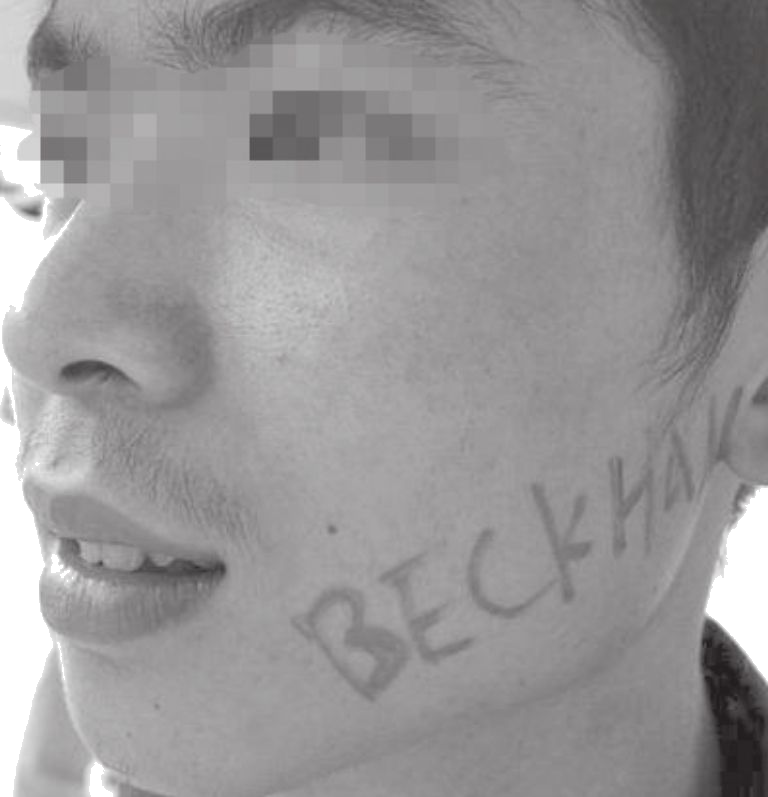
\includegraphics[height=3.5cm]{picture/2006_1.png}
		\caption*{把崇拜写在脸上}
	\end{subfigure}
\hfil
	\begin{subfigure}[b]{0.45\linewidth}
		\centering
		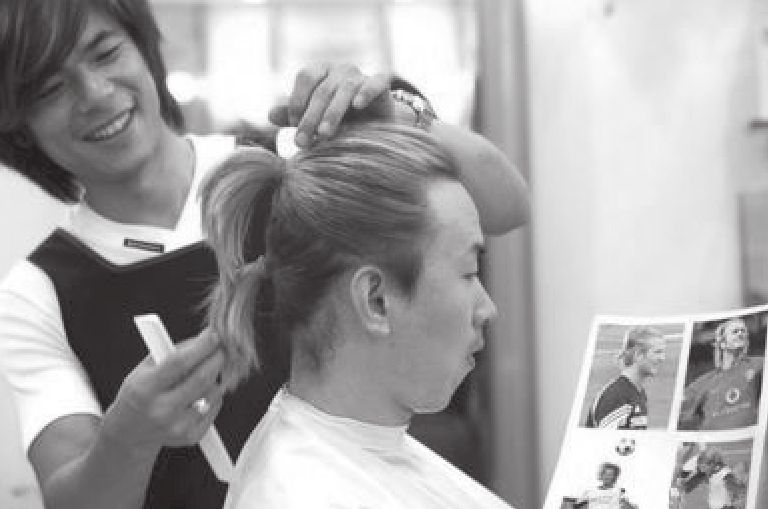
\includegraphics[height=3.5cm]{picture/2006_2.png} 
		\caption*{花300元做个“⼩贝头”}
		\label{fig:2}
	\end{subfigure}
\end{figure}


注:Beckham(贝克汉姆)——英国⾜球明星


\checkpagenumber

